\documentclass{standalone}
\usepackage{tikz}
\begin{document}
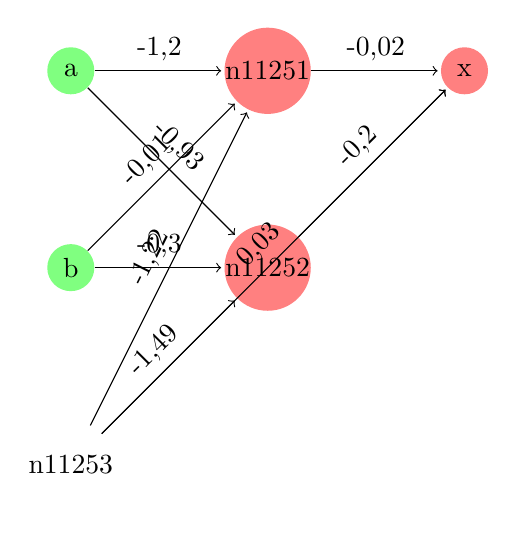
\begin{tikzpicture}[shorten >=1pt,->,draw=black!,node distance=2.5cm]
\tikzstyle{neuron}=[circle,fill=black!25,minimum size=17pt,inner sep=0pt]
\tikzstyle{constant}=[neuron, fill=white!50];
\tikzstyle{identity}=[neuron, fill=green!50];
\tikzstyle{sigmoid}=[neuron, fill=red!50];
\node [identity] (a) {a};
\node [identity,below of=a] (b) {b};
\node [constant,below of=b] (n11253) {n11253};
\node [sigmoid,right of=a] (n11251) {n11251};
\node [sigmoid,below of=n11251] (n11252) {n11252};
\node [sigmoid,right of=n11251] (x) {x};
\path[every node/.style={sloped,anchor=south,auto=false}]
(b) edge node {-0,01} (n11251)
(b) edge node {-0,3} (n11252)
(n11253) edge node {0,03} (x)
(n11253) edge node {-1,22} (n11251)
(n11253) edge node {-1,49} (n11252)
(n11251) edge node {-0,02} (x)
(n11252) edge node {-0,2} (x)
(a) edge node {-0,93} (n11252)
(a) edge node {-1,2} (n11251)
;\end{tikzpicture}
\end{document}